% ---------------------------------------------------------------------------- %
\begin{figure}
	\centering
	\subfigure[\label{fig:linguometer:technical:interference:ex:1}]
	{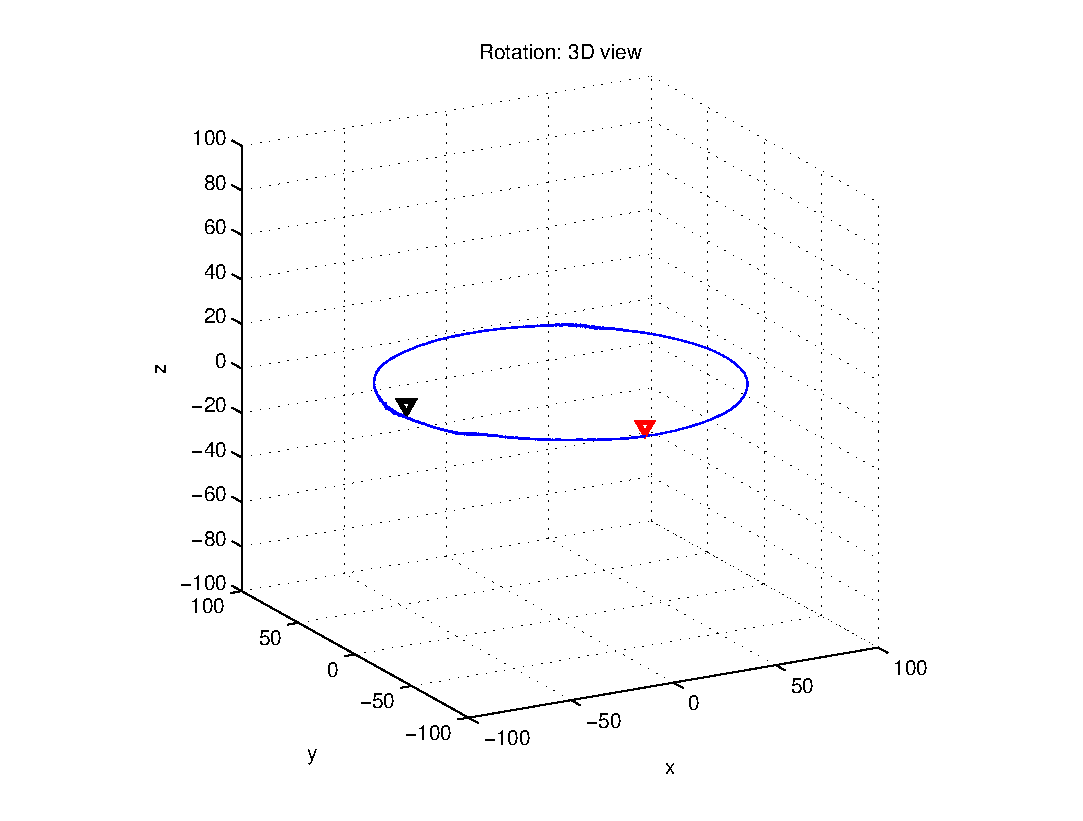
\includegraphics[width=0.45\textwidth]{include/linguometer/images/int_ex_1.eps}}
	\hspace{0.05\textwidth}
	\subfigure[\label{fig:linguometer:technical:interference:ex:2}]
	{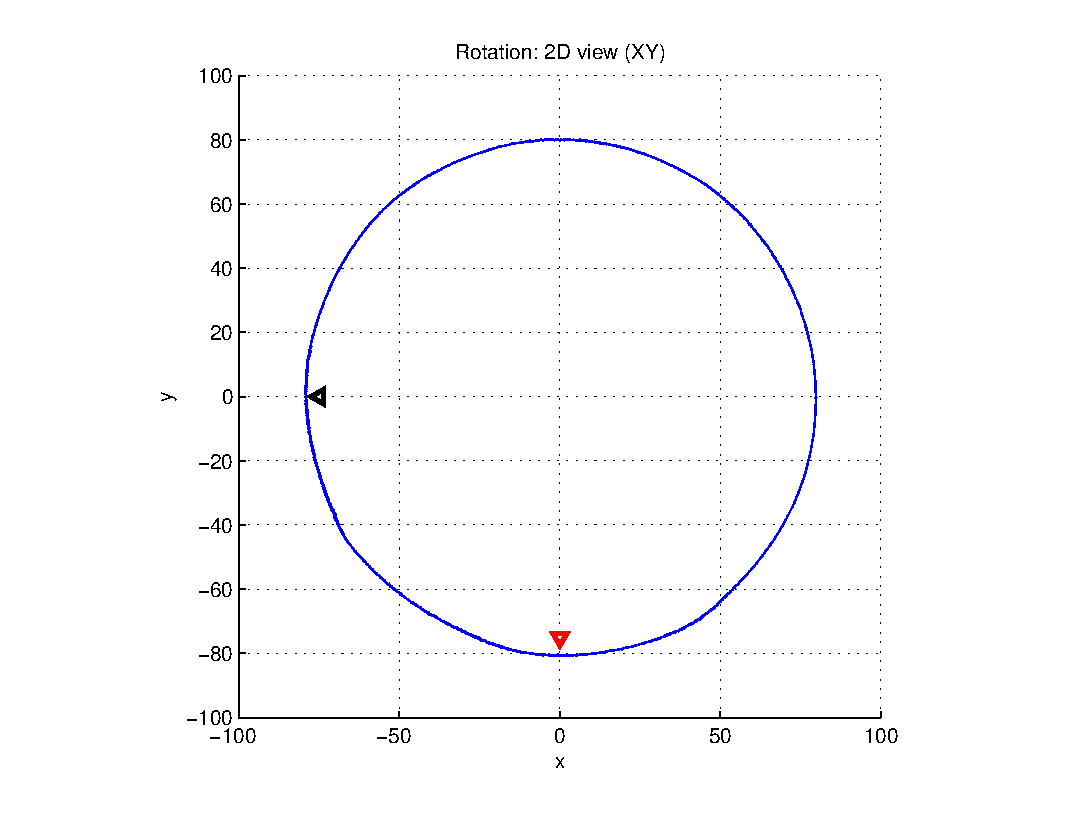
\includegraphics[width=0.45\textwidth]{include/linguometer/images/int_ex_2.eps}}
	
	\subfigure[\label{fig:linguometer:technical:interference:ex:3}]
	{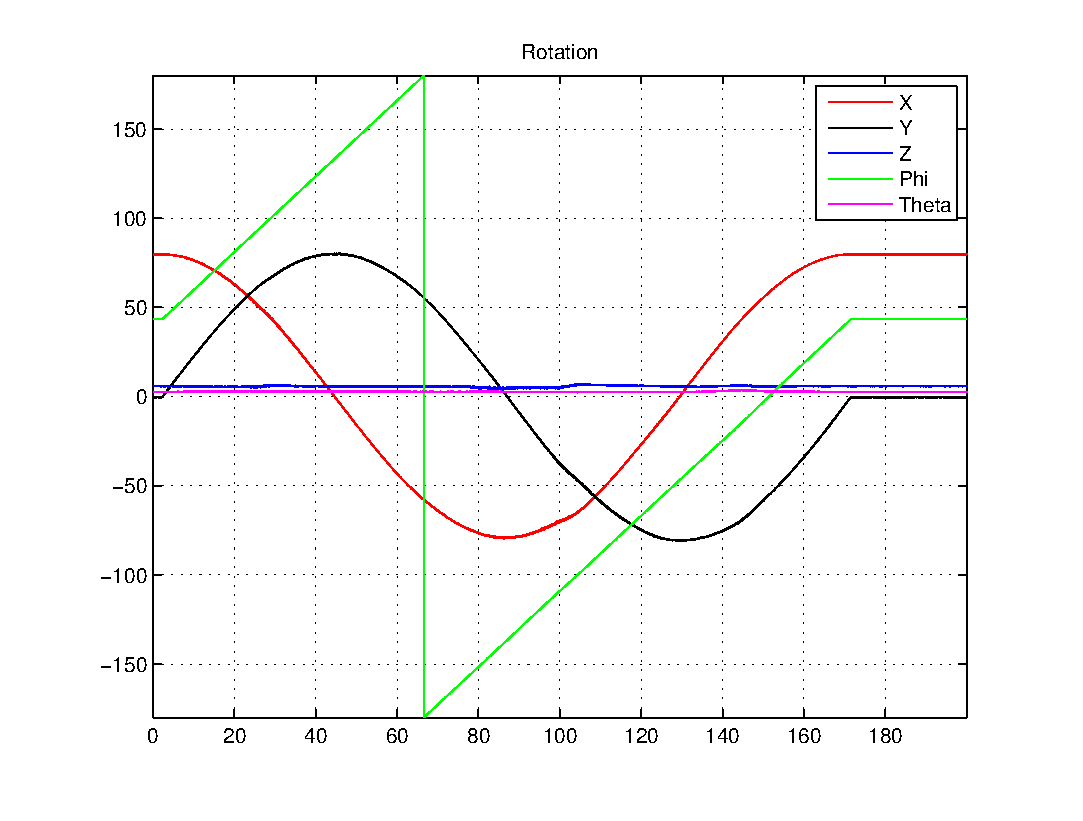
\includegraphics[width=0.45\textwidth]{include/linguometer/images/int_ex_3.eps}}
	\hspace{0.50\textwidth}
	
	\caption[Articulograph sensor rotation]{\textbf{Articulograph sensor
	rotation}: (a) tridimensional view of the rotation of a single sensor
	attached to the AG500 magazines used for calibration. 
	(b) Bidimensional projection (top view) of the previous plot.
	(c) This plot shows the 5DOF acquired by the means of electromagnetic 
	articulography. Three cartesian coordinates (X, Y and Z) and two spherical
	coordinates (Azimuth Tetha and elevation Phi).
	Notes: the red triangle indicates the sensor starting point with respect
	to the XY plane (0 seconds). 
	The black triangle indicates the position of the ultrasonograpic 
	transducer (XY plane).
	The radius of the rotation measures 80 mm while the height at which 
	the rotation takes place measures 6.5 mm. The Theta angle measures circa
	5 $^{\circ}$ and the Phi angle varies during the rotation.
	}
	\label{fig:linguometer:technical:interference:ex}
\end{figure}
% ---------------------------------------------------------------------------- %
